
\subsection{Modelo de presentación}
El modelo de presentación es un diagrama de mapeo, donde se visualizan las interfaces y el mapeo de su navegabilidad del sistema\textbf{QuickContentMedia}.La interfaz del sistema fue diseñada utilizando la herramienta {Figma}~\cite{figma2024}.
\subsubsection{Diagrama de navegabilidad}
Las figuras \ref{fig:mockups} y \ref{fig:mockups2} muestran los mockups relacionados a los casos de uso CU-001 Acceder al portal y CU-010 Administrar Categoría respectivamente.
\begin{figure}[H]
    \centering
    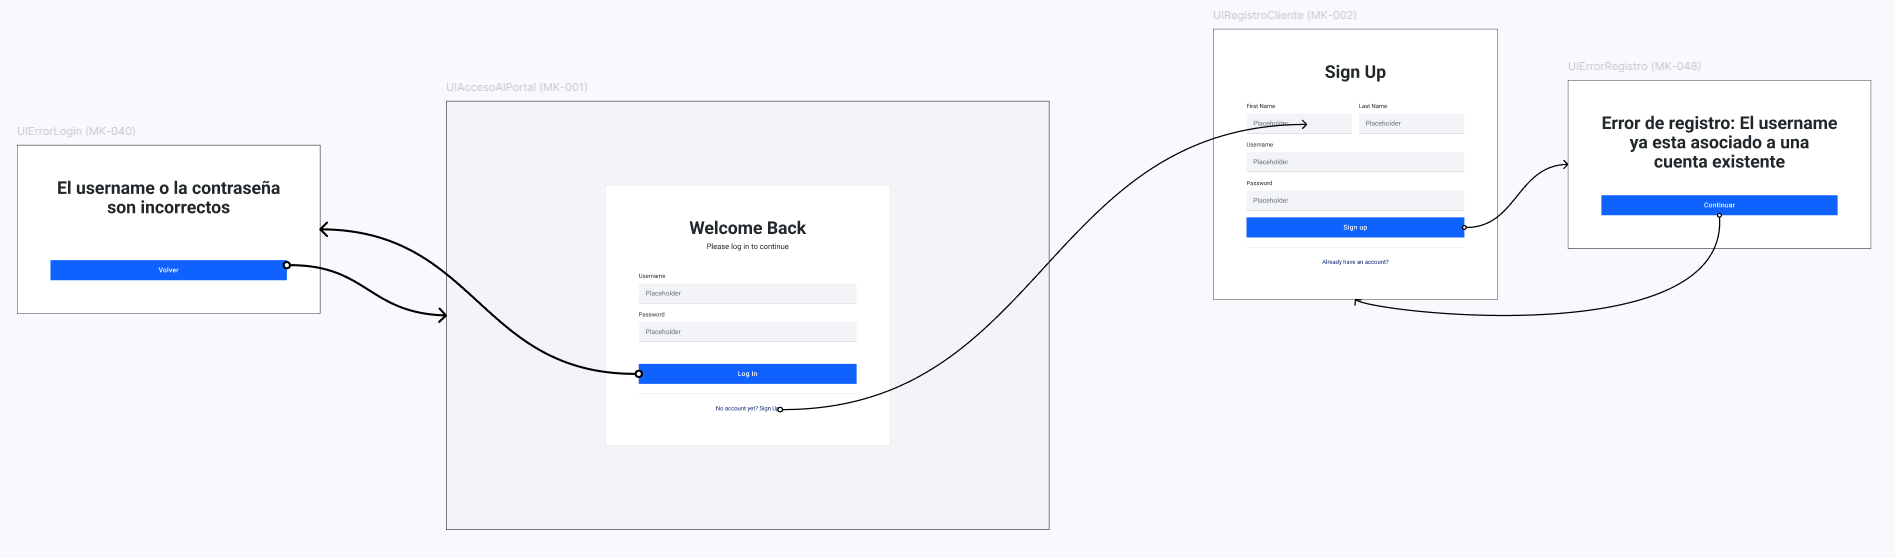
\includegraphics[width=0.95\textwidth]{Media/3_Analisis/3_ModeloDeRequisitos/MK_AccesoAlPortal.png}
    \caption{Mockups relacionados al CU-001 Acceder al portal} 
    \label{fig:mockups}
\end{figure}

\begin{figure}[H]
    \centering
    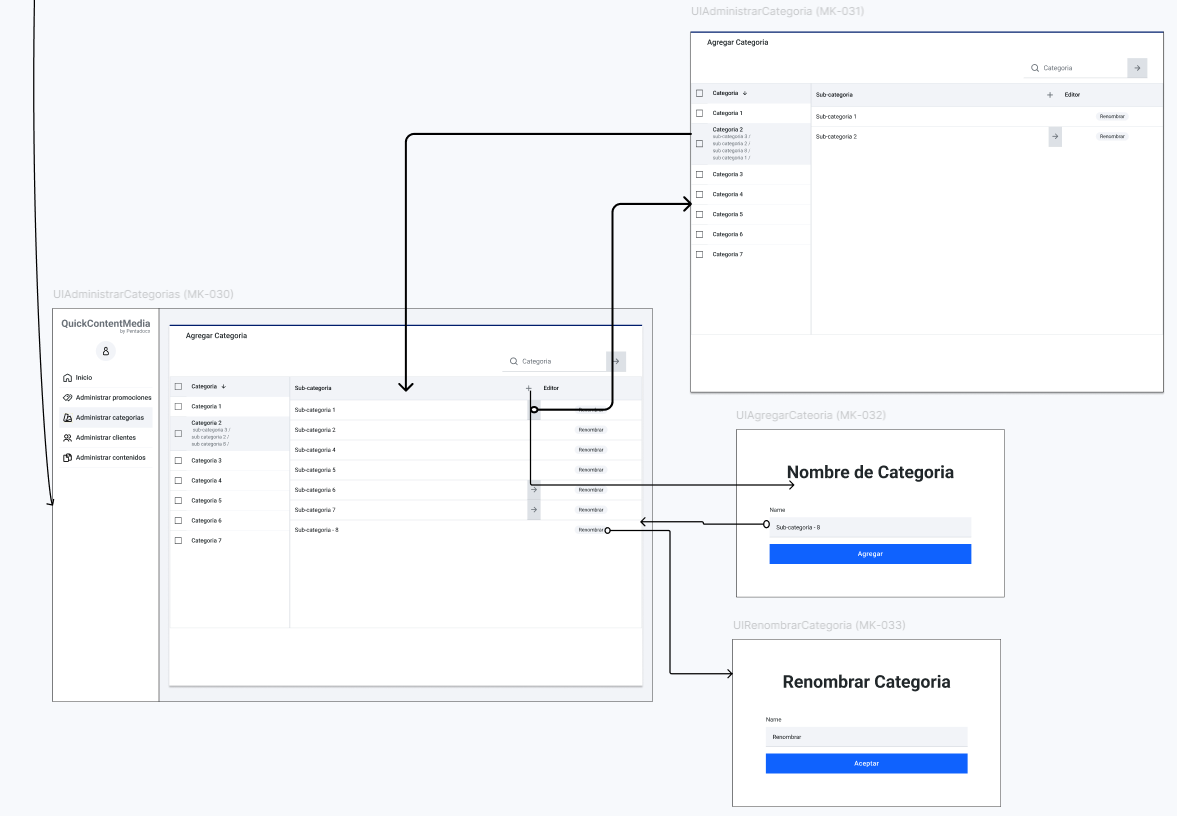
\includegraphics[width=0.95\textwidth]{Media/3_Analisis/3_ModeloDeRequisitos/MK_gestionarCategorias.png}
    \caption{Mockups relacionados al CU-010 Administrar categorías} 
    \label{fig:mockups2}
\end{figure}

\textbf{Documento:} Diagrama de Navegabilidad \\
\textbf{Link de acceso:} \linkDocumentoNavegacion \\

\textbf{Pasos de ejecución:}
\begin{itemize}
    \item Abrir el documento de diagrama de navegabilidad.
    \item Acceder al link de Figma proporcionado dentro del documento.
    \item Visualizar los mockups en Figma.
\end{itemize}